\documentclass[xcolor=table,aspectratio=169]{beamer}

\graphicspath{{figs/}{./figs/}}
\mode<presentation>
{
%  \usetheme{Warsaw}
  \usetheme{Frankfurt}
%  \setbeamercovered{transparent}
  \usecolortheme{crane}
  \setbeamertemplate{navigation symbols}{}
  \setbeamertemplate{section in toc shaded}[default][60]
  \setbeamertemplate{subsection in toc shaded}[default][50]
  \setbeamertemplate{footline}[frame number]
}


\mode<handout>
{
  \beamertemplatesolidbackgroundcolor{black!5}
  \usecolortheme{dove}
%  \usecolortheme{seagull}
}

\usepackage{url}
\usepackage{ulem}
\usepackage{xmpmulti}

% Please add the following required packages to your document preamble:
\usepackage{xcolor}
% If you use beamer only pass "xcolor=table" option, i.e. \documentclass[xcolor=table]{beamer}

\title{Diversity is too important to be left to women}

\author[hmd1]{Hannah Dee \\
  \texttt{hmd1@aber.ac.uk} \\hannahdee.eu} 
\date{}
\institute[]{ACCU 2022,  April 7
  Computer Science, Aberystwyth University\\BCSWomen }



%\beamerdefaultoverlayspecification{<+->}

\AtBeginSection[]
{
  \begin{frame}<beamer>
    \frametitle{Outline}
    \tableofcontents[currentsection,currentsubsection,hideothersubsections]
  \end{frame}
}

\AtBeginSubsection[]
{
  \begin{frame}<beamer>
    \frametitle{Outline}
    \tableofcontents[currentsection,currentsubsection,hideothersubsections]
  \end{frame}
}

\begin{document}

\begin{frame}
  \titlepage
\end{frame}

%%%%%%%%%%%%%%%%%%%%%%%%%%%%%%%%%%%%%%%%%%%%%%%%%%%%%%%%%%%%%%%%%

\section{Intro}

\begin{frame}{What gives me the right to talk about this stuff?}
	\begin{itemize}
		\item Is woman
		\item Is technical
		\item Has read loads of books and articles
		\item On the committee of BCSWomen since 2007
		\item Started the UK's first conference for women undergrads\footnote{\url{https://bcswomenlovelace.bcs.org/}}
	\end{itemize}
\end{frame}
\begin{frame}{What are you going to get out of this talk?}
	\begin{itemize}
		\item An introduction to a bunch of diversity related concepts and terms
		\item Some ranty stuff
		\item Some practical suggestions of things you can do
	\end{itemize}
\end{frame}

\begin{frame}{Karen Sp\"{a}rck Jones} 
	\begin{columns}
		\begin{column}{0.4\textwidth}

	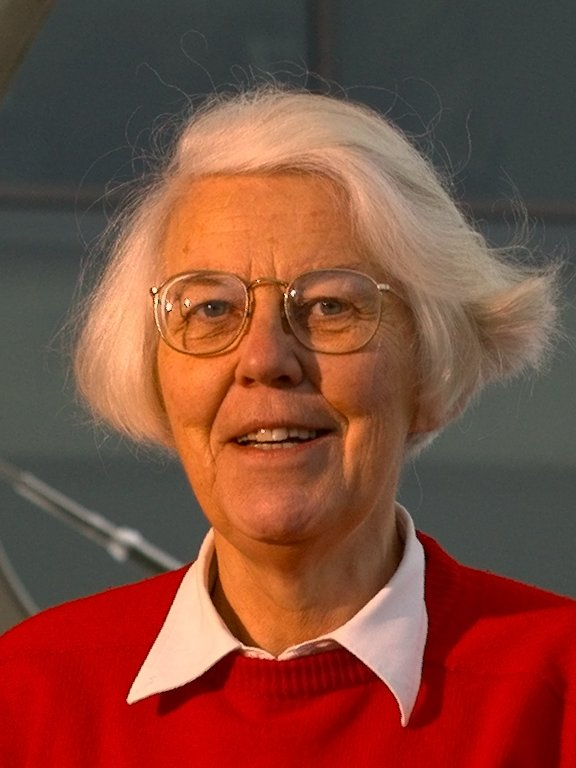
\includegraphics[width=4cm]{ksj.jpg}

	\tiny{University of Cambridge, CC BY 2.5 \url{https://creativecommons.org/licenses/by/2.5}, via Wikimedia Commons}

		\end{column}
		\begin{column}{0.6\textwidth}

		``Computing is too important to be left to men''

			\vspace{0.5em}

			2007
		\end{column}
		\end{columns}
\end{frame}

\begin{frame}{The problem of talking about diversity}

	\begin{columns}
		\begin{column}{0.5\textwidth}
	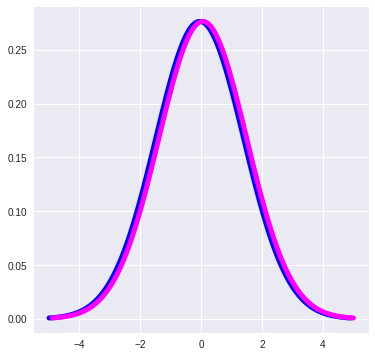
\includegraphics[width=5cm]{gender_diff.png}
		\end{column}
		\begin{column}{0.5\textwidth}
			\sout{Men are from mars, women are from venus} 

			\vspace{0.5em}

			\pause

			People are from earth
		\end{column}
		\end{columns}
\end{frame}

\begin{frame}{General $\rightarrow$ Specific $\rightarrow$ General}

It is simultaneously possible for there to be \ldots

	\begin{itemize}
		\item very little evidence of gender differences in technical ability
		\item some exceptionally talented guys 
		
		\item some really useless women
	\end{itemize}

	The plural of anecdote isn't data

\end{frame}


\begin{frame}{We've come a long way baby}

	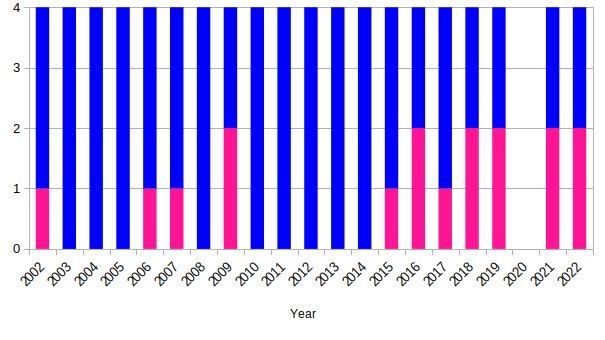
\includegraphics[width=10cm]{accu_key.png}
\end{frame}
\begin{frame}{So isn't diversity in tech a solved problem?}

	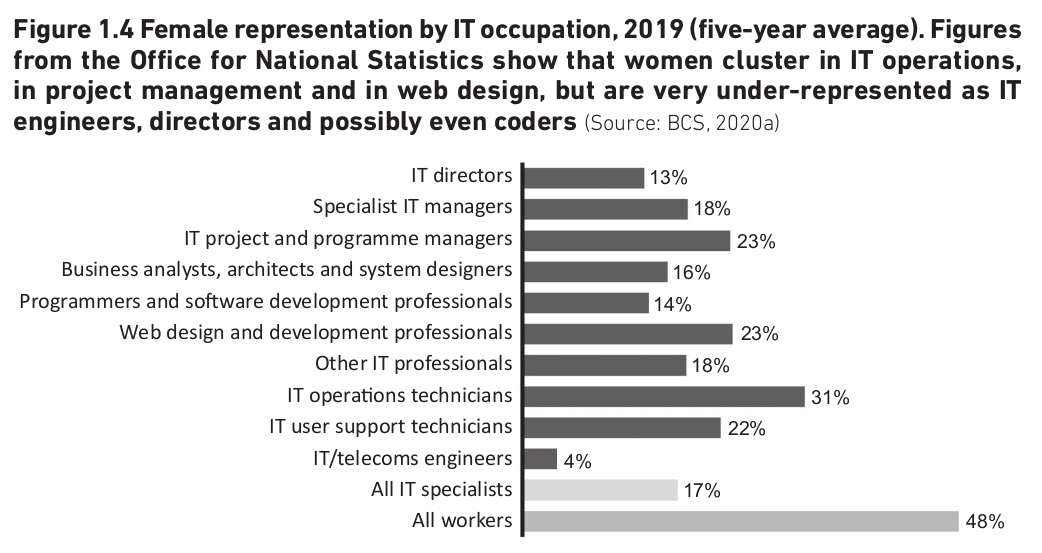
\includegraphics[width=10cm]{it_profession_gender.png}

	\tiny{Source: Women in Tech: A practical guide to increasing gender diversity and inclusion, BCS Publishing \url{https://shop.bcs.org/store/221/detail/workgroup?id=3-221-9781780175614}}
\end{frame}

\begin{frame}{Diversity in tech isn't just gender}

	When there's one clear majority group in a profession, that dominant group's characteristics tend to dominate the profession.  Sociologists talk about``\textbf{Gender role spillover}''  wrt gender imbalances


	\vspace{0.5em}

	Gender is one of the easier characteristics to measure.  	

	\vspace{0.5em}

	Age, disability, gender reassignment, marriage and civil partnership, pregnancy and maternity, race, religion or belief, sex, sexual orientation. Also, class. 


	\vspace{0.5em}


	It's harder to point to a norm, but we need to think about these and also about \textbf{intersectionality}.

\end{frame}
\section{Why}

\begin{frame}{The business case for diversity\ldots}
	\ldots is well-made in a lot of places, recently Financial Reporting council (FRC), 2021, FT350:

More gender diversity generally means 
	\begin{itemize}
		\item better financial performance
		\item less shareholder dissent
		\item more decentralisation in operational practices
		\item more consensus
		\item less overconfidence
	\end{itemize}


	\tiny{\url{https://www.frc.org.uk/getattachment/3cc05eae-2024-45d8-b14c-abb2ac7497aa/FRC-Board-Diversity-and-Effectiveness-in-FTSE-350-Companies.pdf}}
\end{frame}

\begin{frame}{Business motivation}
	\begin{columns}
		\begin{column}{0.5\textwidth}
	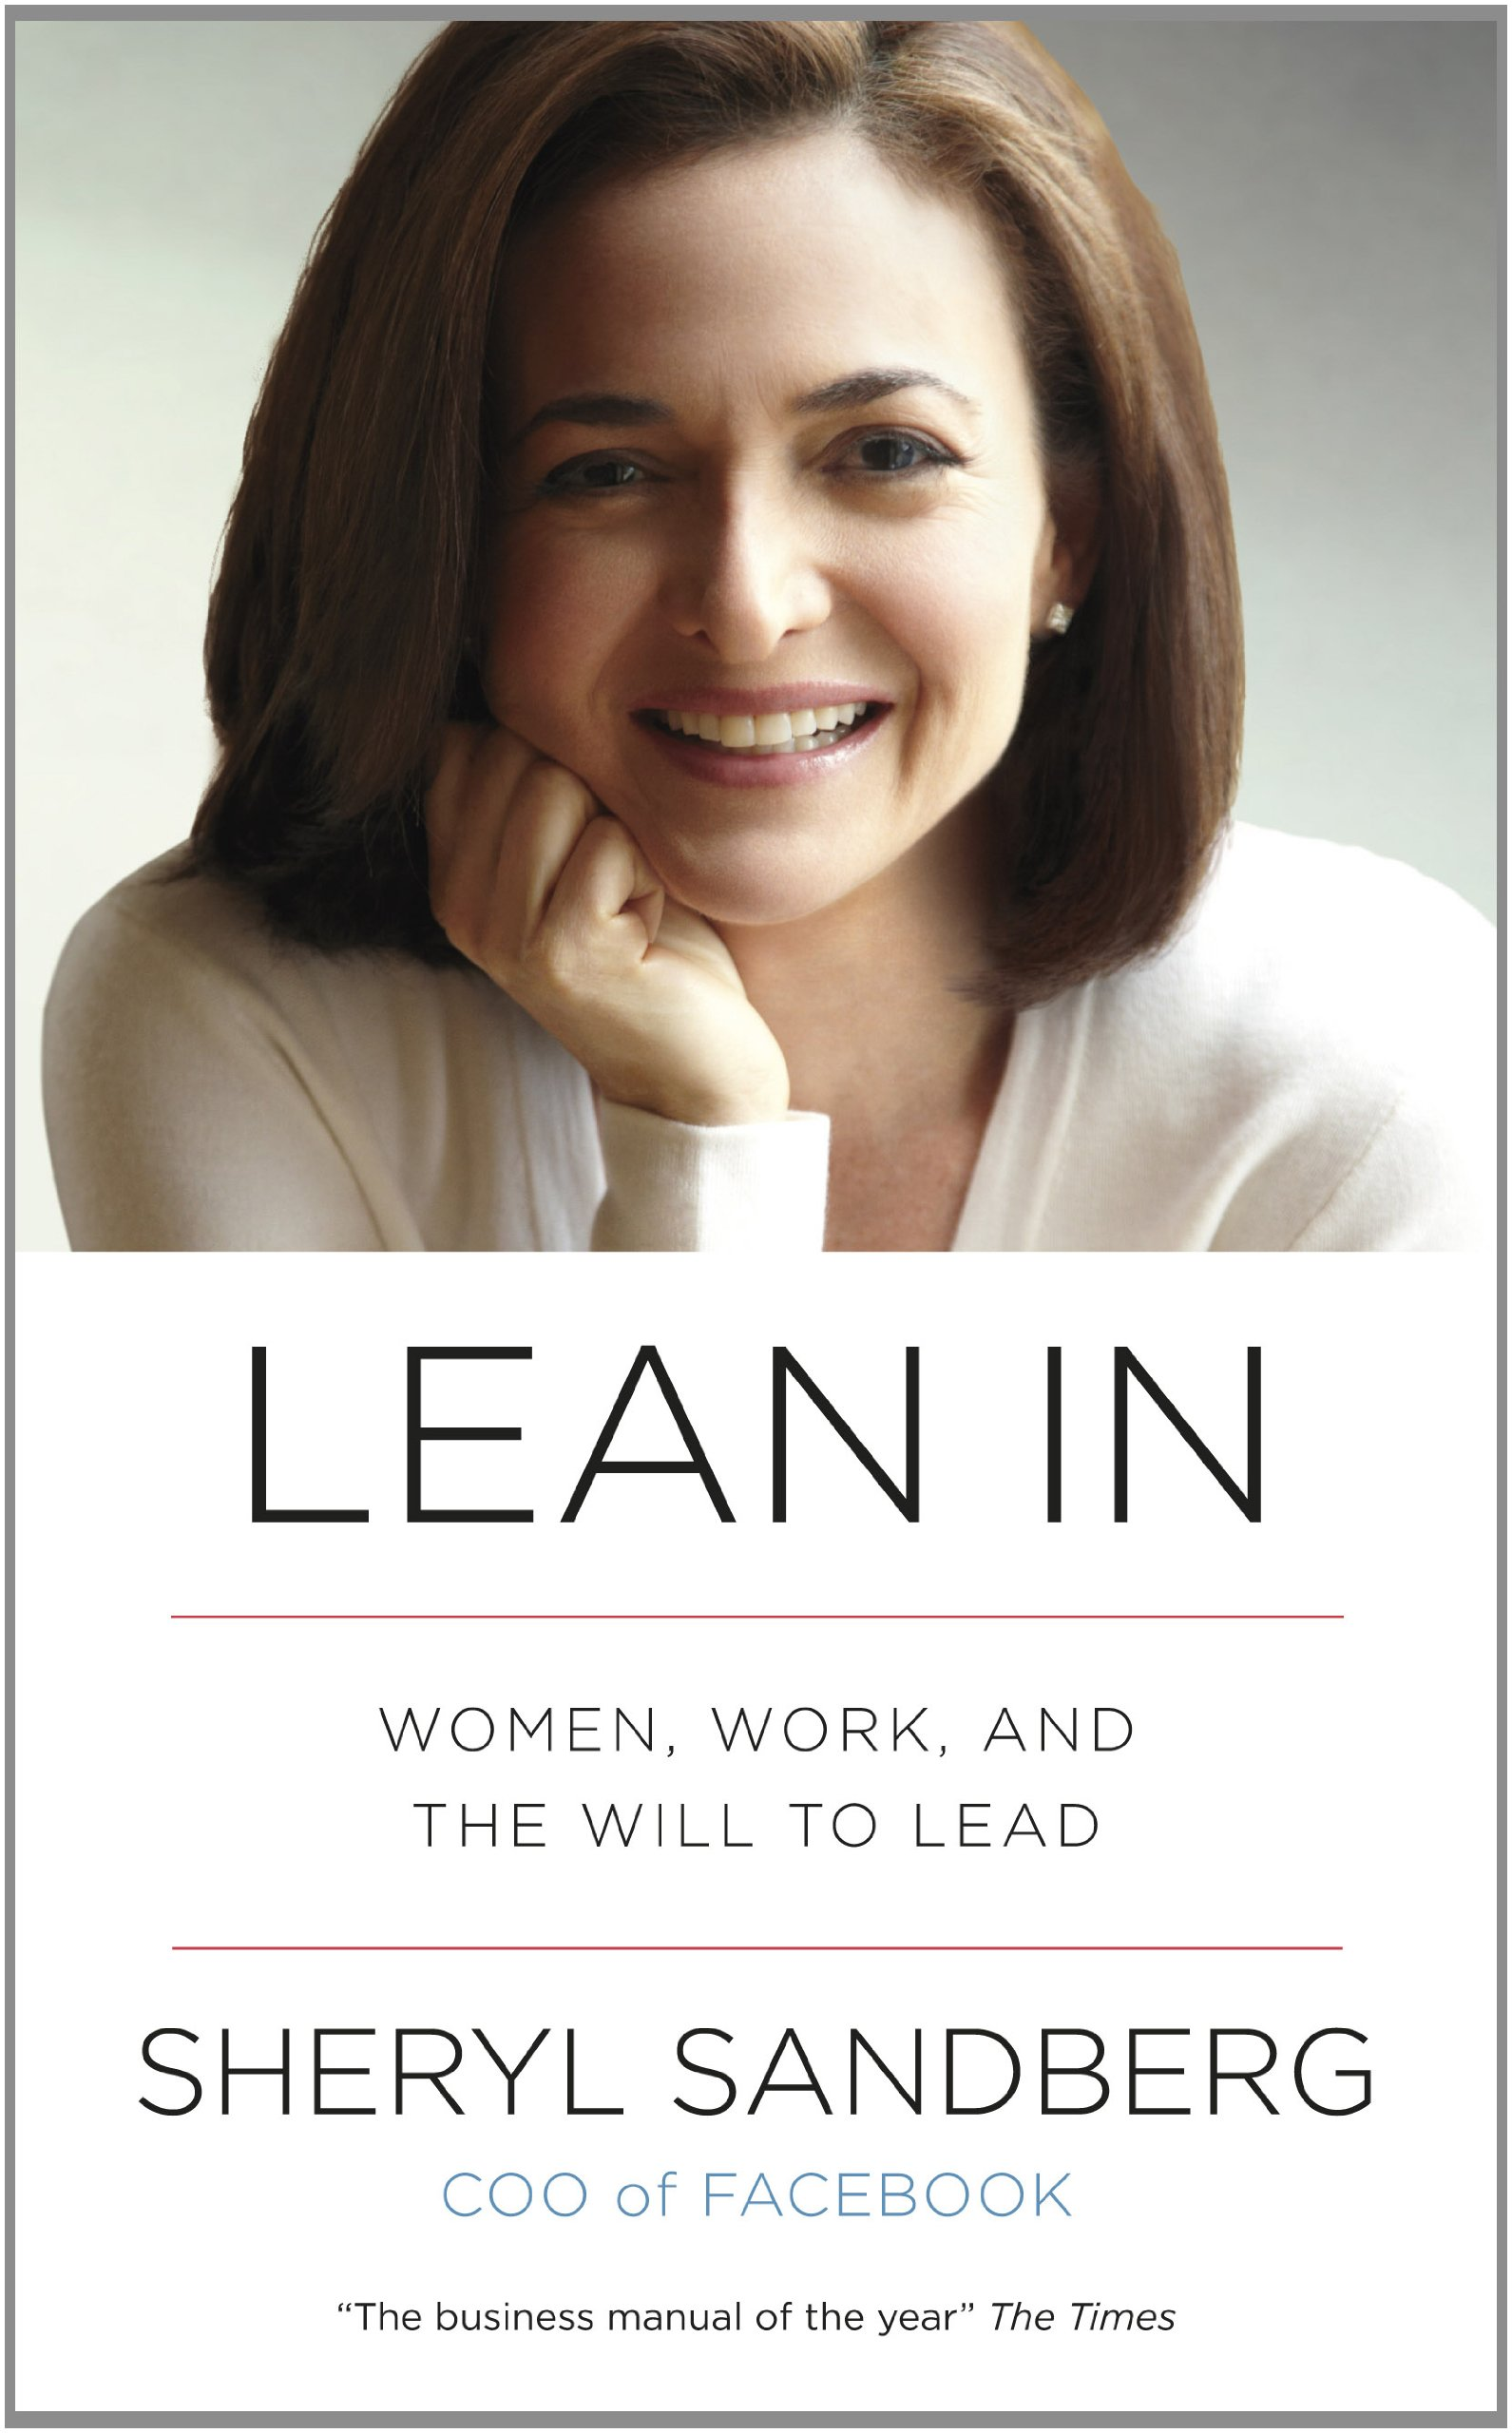
\includegraphics[width=4cm]{lean.jpg}
		\end{column}
		\begin{column}{0.5\textwidth}
			\begin{itemize}
					\pause
				\item Lean In
					\pause
				\item Lean Out
					\pause
				\item Lean sideways?
			\end{itemize}

		\end{column}
	\end{columns}
\end{frame}

\begin{frame}{We design better tech when we consider all the users. }
	\begin{itemize}
		\item Why are Alexa, Cortana and Siri all female voices?
		\item Why have health tracking apps only just started to consider periods?
		\item Voice recognition systems don't work as well with female voices
		\item Face recognition systems don't work as well with Black faces
		\item Why is the first option for gender nearly always Male?
		\item Why do forms still insist gender is binary?
	\end{itemize}
\end{frame}
\begin{frame}{The default male}
	\begin{columns}
		\begin{column}{0.8\textwidth}
	\begin{itemize}
		\item ``If you ask a software engineer what version control they use, he'll say bitbucket.''
		\item ``Here come the beards'' (sorry!)
		\item It's not just tech. Caroline Criado Perez has done a lot of work highlighting this across all fields\footnote{Her newsletter is great: \url{https://carolinecriadoperez.com/}}
			\begin{itemize}
		\item Even nonexistent faces perceived through pareidolia are more likely to be male \footnote{No, really: \url{https://doi.org/10.1073/pnas.2117413119}}
	\end{itemize}
	\end{itemize}
	\end{column}
	\begin{column}{0.2\textwidth}
	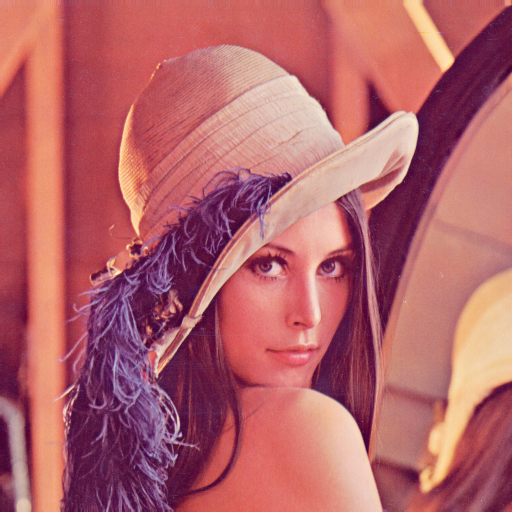
\includegraphics[width=0.8\textwidth]{lena.png}
	\end{column}
	\end{columns}
\end{frame}
\begin{frame}{Pink it and shrink it}
	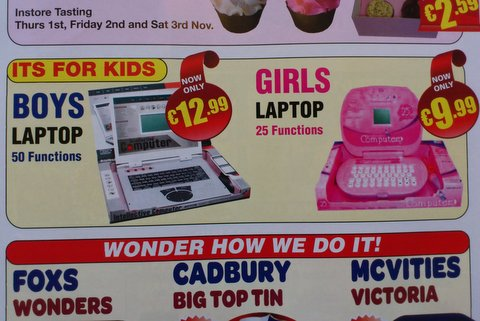
\includegraphics[width=8cm]{laptop_pink.jpg}
\end{frame}
\begin{frame}{Sense of belonging }
	\begin{itemize}
		\item Ever been the only X in the room ?
			\pause
		\item Ever been told to your face that computing isn't for you ?
			\pause
		\item Ever been told you're a good role model?
	\end{itemize}
			\pause
If people do not perceive themselves as belonging in a field, then they're not motivated to join it in the first place, or stay in it. 

\end{frame}

\begin{frame}{Stereotype threat}
	When people are primed to think of themselves as part of a group which is associated with a stereotype, they perform in a way which is more conforming to the stereotype. \footnote{See e.g. \url{https://dx.doi.org/10.1371/journal.pone.0146487}}

	\vspace{0.5em}
	This effect has been shown in 300+ studies across a lot of different domains
	\begin{itemize}
		\item Gender
		\item Race
		\item Socioeconomic group
		\item Age
	\end{itemize}
\end{frame}
\begin{frame}{Self efficacy}
How effective people think they're going to be at a task influences all sorts of aspects of their performance.

	\vspace{0.5em}

There are gender differences in self-efficacy (even?) when controlling for ability \footnote{See e.g. \url{https://link.aps.org/doi/10.1103/PhysRevPhysEducRes.14.020123}}
	\begin{itemize}
		\item Higher self-efficacy leads to better problem solving (less likely to reject correct hypotheses prematurely)
		\item Self-efficacy levels influence choice of task
		\item Self-efficacy levels influence enjoyment of tasks
		\item Self-efficacy levels influence what jobs you apply for
	\end{itemize}
\end{frame}
\begin{frame}{Micro aggressions}
	Leaving aside the macro aggressions (for now) \ldots
	
	\vspace{0.5em}

	The term microaggression makes it seem unimportant

	\begin{itemize}
		\item Hearing demeaning remarks about you
		\item Being mistaken for someone at a lower level
		\item Needing to provide more evidence of your competence
		\item Having your contributions ignored
	\end{itemize}
\end{frame}


\begin{frame}{Being in a minority isn't fun }
	\begin{itemize}
		\item Ever been asked to make the tea?
			\pause
		\item Ever been asked if you can put someone through to the boss?
			\pause
		\item Ever been assumed to be in sales?
	\end{itemize}
	\vspace{0.5em}
But is it inevitable?
\end{frame}

\begin{frame}{Petrie multiplier}
	\transduration<0-71>{0}
	\multiinclude[<+->][format=png, graphics={width=5cm}]{petrie}
				
			Proposed by Karen Petrie, made popular by Ian Gent (who also made the gif).\footnote{Extensions of this have been proposed: \url{https://doi.org/10.1088/1751-8113/48/27/27FT01}}
\end{frame}

\begin{frame}{What does Petrie tell us?}

	\begin{itemize}
		\item Assuming 20\% women the gender ratio is 1:4. 
	        \item There are 4 times as many men so 4 times as many microaggressions are made to women as to men. 
		\item There are also 4 times fewer women available to target, so each individual woman is four times as likely to receive a given remark than an individual man is. 
		\item Therefore: women get 16 times the number of microaggressions. 
		\item This holds: with a gender ratio of $1:r$, women will receive $r^{2}$ times as many microaggressions as men.
	\end{itemize}
\end{frame}


\begin{frame}{Diversity tax}

\begin{itemize}
	\item There are some extra things which women do because they are in a minority in tech
	\item There are some extra things which women do because women are more likely to do some kinds of task
\end{itemize}

\end{frame}

\section{Don't do this}

\begin{frame}{Don't be that guy}

	I'm not going to link to any of the many (many (many)) cases of sexual harassment at tech conferences and in tech companies. Or any of the cases on online harassment.

	\vspace{0.5em}

	Just don't.

\end{frame}

\begin{frame}{Don't hold women and minorities to a higher standard}
	\begin{itemize}
	\item Women shouldn't have to prove their technical credentials
	\item Gate keeping is sometimes useful but more often exclusionary
	\item This applies to women as well as men:
	\begin{itemize}
\item There is evidence that women apply for jobs when meeting more of the criteria\footnote{Although it's not as conclusive as some have argued \url{https://www.bi.team/blogs/women-only-apply-for-jobs-when-100-qualified-fact-or-fake-news/}}
	\end{itemize}
	\end{itemize}
\end{frame}
\begin{frame}{Don't talk over women}

	If men and women talk for equal amounts of time, people report that the women have been talking too much. 

	\vspace{0.5em}

	Measure it: \url{http://arementalkingtoomuch.com/}


	\vspace{0.5em}


	Don't talk over women

\end{frame}
\begin{frame}{Don't pay women less}

	Anyone here on twitter?

	\vspace{0.5em}

	Anyone here enjoy Pay Gap Bot on March 8? \url{https://twitter.com/PayGapApp}
\end{frame}

\section{Do do this}

\begin{frame}{Be an ally}

	Minorities are told they don't belong, are dealing with stereotype threat, micro-aggressions, and macro-aggressions.

	\vspace{0.5em}

	They could do with some support.

\end{frame}
\begin{frame}{The really easy stuff}
	\begin{itemize}
		\item Amplify women's voices
		\item Pledge: never appear on a manel
		\item Pledge: never appear at an event without a CoC
		\item Encourage women and girls : ``you can do this''
		\item Talk about your salary
		\item Learn about unconscious bias
	\end{itemize}
\end{frame}
\begin{frame}{Learn about the law}
	A new thing: Discrimination first aider\footnote{\url{https://valla.uk/discrimination-first-aid-training}}. 
	
	\vspace{0.5em}

	This is first aid for people who are experiencing discrimination - exactly as it says on the tin. 
	
	\vspace{0.5em}


	It covers things you might need to know as a first responder in a crisis, supporting a victim of discrimination: practical resources to address the issue, evidence gathering, legal information, and informed emotional support.



\end{frame}

\begin{frame}{Consider workload}
	\begin{itemize}
		\item There's a workload associated with being in a minority
		\item \textbf{Diversity tax}
		\item Mentoring, panels, speaking, pastoral care
		\item Also: actual extra work 
		\item (This is ignoring the shadow workload of harassment tribunals, equal pay appeals, and discrimination cases)
	\end{itemize}
	If you're a manager, can you take this into account?  
\end{frame}

\begin{frame}{Volunteer}
        Pick up some of the diversity work. 
	\begin{itemize}
		\item Make sure the events you organise are safe for minorities
		\item Help organise events for minority groups
		\item Mentor and sponsor people from minority groups\footnote{\url{https://hbr.org/2021/06/dont-just-mentor-women-and-people-of-color-sponsor-them}} 
			\begin{itemize}
				\item Your mentor can be a peer, or someone junior
				\item Sponsors advocate on your behalf
			\end{itemize}
		\item Don't leave women to do the pastoral stuff 
	\end{itemize}
\end{frame}
\begin{frame}{Consider the personal cost of activities}
	\begin{itemize}
		\item Events after work or at weekends aren't accessible to all
		\item Refunding work travel after the fact can be problematic for those with financial constraints
	\item Travel can be hard for those with caring responsibilities
	\item Some countries can be dangerous for LGBT+ colleagues, or those from ethnic minorities
	\end{itemize}
\end{frame}
\begin{frame}{Consider sense-of-belonging}
One way to feel like you're not alone as a women in tech is to go to women in tech events 

	\vspace{0.5em}

	If you have women staff, provide time for them to do this (and travel, if needed)
\end{frame}

\begin{frame}{Consider homogenisation}
	\begin{itemize}
		\item Not every woman wants to get involved in diversity stuff.
		\item Not every gay person wants to go to Pride
		\item Not every Asian colleague will be observing Ramadan right now. 
		\item Not every colleague observing Ramadan right now will be Asian.  
	\end{itemize}
\end{frame}

\begin{frame}{Foster self-efficacy}

	This goes for all people - but particularly minorities

	\vspace{0.5em}

	Confidence is really hard to build up and really easy to knock

	\vspace{0.5em}

	Compliments are cheap: be excellent to each other. If someone's done a good job, tell them. If someone's not sure they can do something (and you think they can), tell them.

\end{frame}
\begin{frame}{Foster a sense of belonging}

	You belong here, I belong here, we all belong here 

	\vspace{0.5em}

	People should be able to bring their whole selves to work

	\vspace{0.5em}

Think about: catering, holidays, caring responsibilities, accessible spaces. 
\end{frame}


\section{Conclusions}
	\begin{frame}{We all need to take diversity seriously}
		\begin{itemize}
		\item It's bad for tech, business, minorities and majorities 
		\item Women can't fix it on our own
		\begin{itemize}
			\item It's bad for us
			\item It's bad for our careers
			\item It's bad for tech
		\end{itemize}
	\end{itemize}
	\end{frame}

\begin{frame}{What's good for the gander is good for the goose}
	``A profession that's better for women is good for all'' - Rebecca George 

	\begin{itemize}
		\item Better business
		\item More, happier, diverse workforce
		\item Better conditions
	\end{itemize}
	\vspace{0.5em}

	Also, we've been trying to solve this for ages and we've not succeeded! We need your massive brains to help us crack this one.

\end{frame}


\begin{frame}{Any questions?}

	\begin{itemize}
	\item Questions?
	\item Thoughts?
	\item Disagreements?
	\end{itemize}
\end{frame}


\end{document}
